\chapter{DÉPLOIEMENT}


Pour la réalisation et la mise en place de la solution, il a été nécessaire de recourir à un certain nombre d’outils et mettre en place des environnements d’exécution.
Ce chapitre a pour objectif, de décrire l’environnement mis en place et les outils utilisés, ainsi que de décrire l’environnement existant (matériels et logiciels), et dans lequel évoluera notre système.

\section{PARTIE WEB}
 Cette partie est celle qui sera accessible depuis la plateforme en ligne. Elle couvre les différents besoins exprimés pour les profils client, hôteliers et administrateurs. Elle sera réalisée sur le système de Hosteline. Ainsi, la finalité de cette mise en œuvre sera un système décisionnel qui fonctionne côte à côte avec le système opérationnel. Le diagramme de la figure qui suit est fait selon les formalismes du diagramme de déploiement spécifié plus haut. Il décrit le système mis en place pour cette partie.
 
\begin{figure}[!htbp]
	\begin{center}
		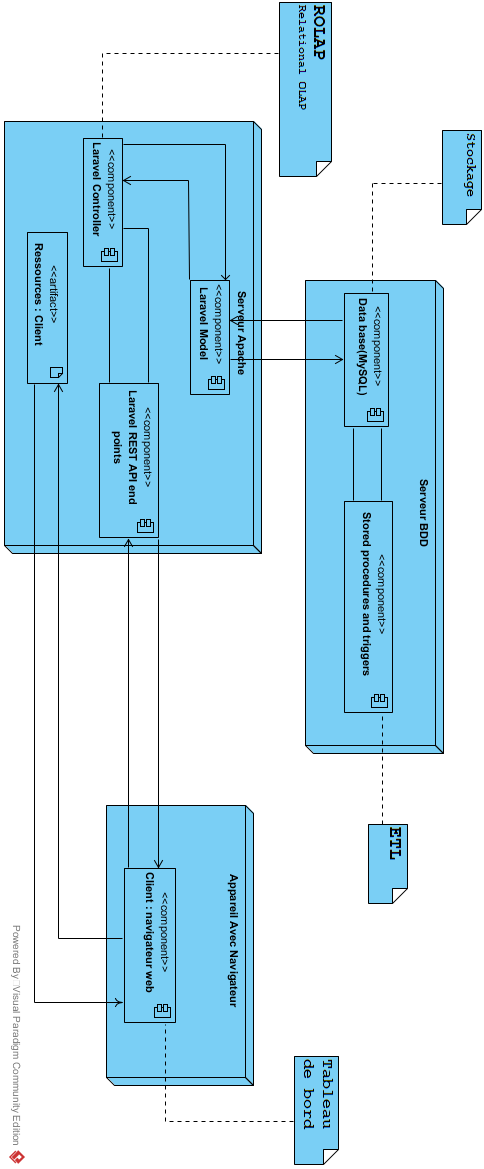
\includegraphics[scale=0.75]{images/deploy_web.png}
	\caption{Diagramme de déploiement de la partie web}
		\label{use_case_diagramme_one}
	\end{center}
\end{figure}

\cleardoublepage
\section{PARTIE DESKTOP}
Cette partie sera installé en local a l’entreprise sur une machine prévu a cette effet. C’est sur cette machine que sera installée la suite Pantaho. Le diagramme de la figure suivant explique comment ce système est mis en œuvre.

\begin{figure}[!htbp]
	\begin{center}
		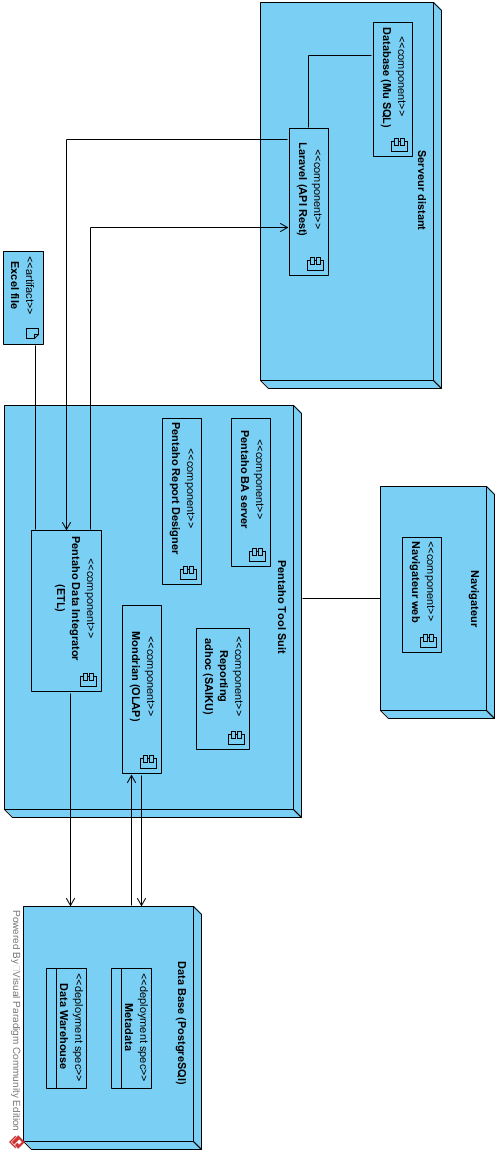
\includegraphics[scale=0.65]{images/deploy_desktop.png}
	\caption{Diagramme de déploiement de la partie desktop}
		\label{use_case_diagramme_one}
	\end{center}
\end{figure}





